\chapter{Sliding Window Flash Attention}\label{ch:swfa}

\emph{Placement in the stack.} Chapter~\ref{ch:cutlass} showed
that the skinny attention-score GEMM is the single most
under-utilised shape class in a transformer forward pass. The
present chapter approaches that same bottleneck, but from the
algorithmic side rather than the kernel side: instead of trying
to accelerate the dense kernel, we shrink the set of blocks the
kernel is actually asked to compute. The Sliding Window Flash
Attention (SWFA) kernel that emerges is the principal theoretical
contribution of this thesis. Its correctness proof
(Appendix~\ref{app:proofs_classify}) and its closed-form
expression for the optimal window size
(Appendix~\ref{app:proof_optw}) are treated rigorously in what
follows. SWFA is then picked up again in two later chapters: in
Chapter~\ref{ch:sglang} as the prefill kernel of the SGLang
runtime, and in Chapter~\ref{ch:triton} as the cross-validation
target of the Triton port.

\section{Motivation}\label{sec:swfa_motivation}
The cost of attention scales as $N^2$ in the sequence length, and
at the context sizes that current production models operate at
($N \geq 8{,}192$) it is this quadratic term that sets both the
training throughput and the decode latency. The Flash Attention
line of work~\cite{dao2022flashattention,dao2023flashattention2}
relieves the \emph{memory} side of the quadratic cost by streaming
the attention computation in tiles, but it still issues a dense
GEMM for every $B_r \times B_c$ tile, including those that the
model is about to mask out. Many long-context models restrict the
attention pattern to a local window on architectural
grounds~\cite{beltagy2020longformer,zaheer2020bigbird}, so that a
query at position $i$ is only allowed to attend to keys in the
range $[i - w_l,\, i + w_r]$. Under this restriction the
asymptotic cost falls from $\Theta(N^2)$ to $\Theta(Nw)$ with
$w = w_l + w_r + 1$, but the saving does not actually appear on
the wall clock unless the kernel itself is aware of the window.

This chapter introduces \emph{Sliding Window Flash Attention}
(SWFA), which combines Flash Attention's block-wise computation
with a preprocessing step that classifies each attention block
into one of three sets: fully inside the window, intersecting it,
or lying entirely outside. Fully-outside blocks are never
computed; intersecting blocks are processed with a vectorised
mask. In practice the algorithm skips up to $65.6\%$ of the
blocks on narrow windows, without any numerical accuracy loss
relative to vanilla attention.

\section{Background}\label{sec:swfa_background}

\subsection{Flash Attention}\label{sec:fa_bg}
The standard form of attention,
\begin{equation}
\mathrm{Attention}(Q, K, V) =
\mathrm{softmax}\!\left(\frac{Q K^{\!\top}}{\sqrt{d}}\right) V ,
\end{equation}
is written as three operations---scores, softmax, output---and
naturally produces an intermediate score matrix of size
$N \times N$. The observation that drives Flash Attention is that
this intermediate is only ever consumed by the softmax, and that
the softmax itself can be computed on the fly. If the queries are
partitioned into row tiles of height $B_r$ and the keys and values
into column tiles of width $B_c$, a running pair of row-max and
row-sum, $(m_i, \ell_i)$, is sufficient to re-scale the previously
accumulated contributions every time a new column tile arrives:
\begin{equation}\label{eq:online_softmax}
m_i^{\text{new}} = \max(m_i, \max_j s_{ij}),\quad
\ell_i^{\text{new}} = e^{m_i - m_i^{\text{new}}} \ell_i
                     + \sum_j e^{s_{ij} - m_i^{\text{new}}} ,
\end{equation}
A matching correction factor is then applied to the output
accumulator $O_i$. Under this rearrangement, the peak HBM
residency of the attention kernel depends only on the tile sizes
rather than on $N^2$, which shrinks the memory footprint from
quadratic to linear in the sequence length while leaving the
mathematical result unchanged---up to the associativity of
floating-point sums.

\subsection{Sliding-Window Attention}\label{sec:sw_bg}
A symmetric window of size $w$ keeps only those attention weights
whose key position $j$ lies within $w/2$ of the query position
along the diagonal, i.e.\ those satisfying
\begin{equation}\label{eq:window}
\max(0, i - w_l) \leq j \leq \min(N-1, i + w_r).
\end{equation}
In existing implementations, this constraint is applied as an
element-wise mask \emph{after} the attention scores have been
computed---wasteful, because entire $B_r \times B_c$ blocks can
sit outside the band and still pay the full dense GEMM cost. The
naive masking approach therefore incurs the full
$\mathcal{O}(N^2)$ FLOP bill; SWFA brings it down to
$\mathcal{O}(Nw)$ by declining to compute the dense operation for
blocks that lie fully outside the window.

\section{Method}\label{sec:swfa_method}

\subsection{Block Classification}\label{sec:swfa_classify}
Given a sequence length $N$, block sizes $(B_r, B_c)$, and the
window parameters $(w_l, w_r)$, the attention matrix is first
partitioned into a $T_r \times T_c$ grid of blocks with
\begin{equation}
T_r = \left\lceil \frac{N}{B_r} \right\rceil, \qquad
T_c = \left\lceil \frac{N}{B_c} \right\rceil .
\end{equation}
Each block $(r, c)$ then falls into exactly one of three sets:
\begin{description}
    \item[$\mathcal{I}$ (fully inside).] Every $(q, k)$ pair in
          the block satisfies~\eqref{eq:window}; no mask is
          needed.
    \item[$\mathcal{X}$ (intersecting).] Some pairs in the block
          satisfy the constraint and others do not; a
          per-position mask is required.
    \item[$\mathcal{O}$ (fully outside).] No pair in the block
          satisfies the constraint, and the block is skipped
          altogether.
\end{description}

Figure~\ref{fig:swfa_classify} illustrates these three classes on
an $8 \times 8$ attention grid with $w_l = w_r = 2$, using
$B_r = B_c = 1$ for clarity. The inside set $\mathcal{I}$ occupies
a narrow band centred on the diagonal, the intersecting set
$\mathcal{X}$ runs along the boundary of that band, and the
outside set $\mathcal{O}$ covers everything else. Only the blocks
in $\mathcal{I} \cup \mathcal{X}$ ever enter the kernel loop, and
of those, only the $\mathcal{X}$ blocks actually need the
vectorised mask produced by Algorithm~\ref{alg:swfa_mask}.

\begin{figure}[H]
    \centering
    \begin{tikzpicture}[
        cell/.style={minimum width=6mm, minimum height=6mm, draw=black!40,
                     inner sep=0pt, font=\tiny},
        inside/.style ={cell, fill=green!40},
        inter/.style  ={cell, fill=orange!50,
                        pattern=north east lines, pattern color=orange!80!black},
        outside/.style={cell, fill=gray!12},
        arr/.style={-latex}
    ]
    % 8x8 grid; rows = query index i (top=0, bottom=7),
    % cols = key index j (left=0, right=7); window |i-j| <= 2
    \foreach \i in {0,...,7} {
        \foreach \j in {0,...,7} {
            \pgfmathtruncatemacro{\diff}{abs(\i - \j)}
            \ifnum\diff=0
                \node[inside]  at (\j*6mm, -\i*6mm) {};
            \else\ifnum\diff=1
                \node[inside]  at (\j*6mm, -\i*6mm) {};
            \else\ifnum\diff=2
                \node[inter]   at (\j*6mm, -\i*6mm) {};
            \else
                \node[outside] at (\j*6mm, -\i*6mm) {};
            \fi\fi\fi
        }
    }
    % axis labels
    \foreach \j in {0,...,7}
        \node[font=\tiny] at (\j*6mm, 4mm) {\j};
    \foreach \i in {0,...,7}
        \node[font=\tiny] at (-4mm, -\i*6mm) {\i};
    \node[font=\scriptsize, anchor=south] at (21mm, 8mm) {key index $j$};
    \node[font=\scriptsize, rotate=90, anchor=south] at (-9mm, -21mm)
        {query index $i$};

    % Legend
    \node[inside,  label=right:{\scriptsize $\mathcal{I}$ (inside)}]
        at (60mm,   0mm) {};
    \node[inter,   label=right:{\scriptsize $\mathcal{X}$ (intersecting)}]
        at (60mm,  -8mm) {};
    \node[outside, label=right:{\scriptsize $\mathcal{O}$ (skipped)}]
        at (60mm, -16mm) {};
    \draw[arr, thick] (85mm, -30mm) -- (85mm, -38mm);
    \node[font=\scriptsize, align=left, anchor=north] at (85mm, -38mm)
        {only $\mathcal{I}\cup\mathcal{X}$\\ enters the kernel};
    \end{tikzpicture}
    \caption{SWFA block classification on an $8 \times 8$ grid with
             window $w_l = w_r = 2$. Green cells ($\mathcal{I}$)
             require no masking; hatched orange cells ($\mathcal{X}$)
             receive the vectorised mask of
             Algorithm~\ref{alg:swfa_mask}; grey cells
             ($\mathcal{O}$) are skipped entirely. The skipped
             fraction grows quadratically with $N/w$, yielding the
             $1 - 2w/N$ asymptotic ratio proved in
             Appendix~\ref{app:proofs_block}.}
    \label{fig:swfa_classify}
\end{figure}

Algorithm~\ref{alg:swfa_classify} performs the classification by
examining the block corners.

\begin{algorithm}[h]
    \caption{Block classification for the sliding window.}
    \label{alg:swfa_classify}
    \KwIn{Sequence length $N$, window $(w_l, w_r)$, block sizes
          $(B_r, B_c)$.}
    \KwOut{Sets $\mathcal{I}$, $\mathcal{X}$, $\mathcal{O}$ of block
           indices.}
    $T_r \leftarrow \lceil N/B_r \rceil,\ T_c \leftarrow \lceil N/B_c
       \rceil$\;
    $\mathcal{I}, \mathcal{X}, \mathcal{O} \leftarrow \emptyset$\;
    \For{$r = 0$ \KwTo $T_r - 1$}{
        row\_start $\leftarrow r\,B_r$,\
        row\_end $\leftarrow \min((r+1)B_r, N)-1$\;
        \For{$c = 0$ \KwTo $T_c - 1$}{
            col\_start $\leftarrow c\,B_c$,\
            col\_end $\leftarrow \min((c+1)B_c, N)-1$\;
            $L_{\text{top}} \leftarrow \max(0, \text{row\_start}-w_l)$\;
            $R_{\text{top}} \leftarrow \min(N-1, \text{row\_start}+w_r)$\;
            $L_{\text{bot}} \leftarrow \max(0, \text{row\_end}-w_l)$\;
            $R_{\text{bot}} \leftarrow \min(N-1, \text{row\_end}+w_r)$\;
            outside $\leftarrow (\text{col\_end} < L_{\text{top}})$ or
                               $(\text{col\_start} > R_{\text{bot}})$\;
            inside  $\leftarrow (\text{col\_end} \le R_{\text{top}})$ and
                               $(\text{col\_start} \ge L_{\text{bot}})$\;
            \uIf{outside}{$\mathcal{O} \leftarrow
                \mathcal{O} \cup \{(r,c)\}$}
            \uElseIf{inside}{$\mathcal{I} \leftarrow
                \mathcal{I} \cup \{(r,c)\}$}
            \Else{$\mathcal{X} \leftarrow
                \mathcal{X} \cup \{(r,c)\}$}
        }
    }
    \Return $\mathcal{I}, \mathcal{X}, \mathcal{O}$\;
\end{algorithm}

\subsection{Correctness of the Classifier}\label{sec:swfa_classify_proof}
\begin{lemma}[Corner-check sufficiency]\label{lem:corner}
Let $B = [r_0, r_1] \times [c_0, c_1]$ be an axis-aligned block of the
attention matrix, and let
$W = \{(i, j) : i - w_l \le j \le i + w_r\}$ denote the window band.
Then:
\begin{enumerate}
    \item[\textup{(i)}]
    $B \cap W = \emptyset \iff c_1 < r_0 - w_l \text{ or } c_0 > r_1 + w_r$;
    \item[\textup{(ii)}]
    $B \subseteq W \iff c_1 \le r_0 + w_r \text{ and } c_0 \ge r_1 - w_l$.
\end{enumerate}
\end{lemma}
\begin{proof}
The window is the strip between the two lines $j = i - w_l$ (lower
boundary) and $j = i + w_r$ (upper boundary). Because these boundaries
are monotone in $i$, the minimum of $j - i$ over $B$ is attained at
$(r_1, c_0)$ and the maximum at $(r_0, c_1)$. The block lies entirely
outside $W$ iff the minimum of $j - (i + w_r)$ is positive over $B$
or the maximum of $j - (i - w_l)$ is negative, which are exactly the
two conditions stated; similarly, the block lies entirely inside $W$
iff both extrema of $j - i$ fall inside $[-w_l, w_r]$. Clipping at
$[0, N-1]$ does not affect the inequalities because the window
intersected with $[0, N-1]^2$ is a subset of the unclipped band.
\end{proof}

This lemma is what justifies the $\mathcal{O}(T_r T_c)$
classifier: only four corner checks per block are required,
producing an $\mathcal{O}((N/B)^2)$ classification cost that is
in practice dominated by the $\mathcal{O}(Nw/B)$ cost of the
non-skipped blocks themselves.

\subsection{Vectorised Mask Generation}\label{sec:swfa_mask}
For a block $(r, c)$, define the block diagonal offset
$\delta_{rc} = c B_c - r B_r$. A local position $(i_\ell, j_\ell)$
inside the block corresponds to relative position
$\mathrm{rel} = j_\ell - i_\ell$, which must be masked whenever
\begin{equation}
    \mathrm{rel} > w_r + \delta_{rc}
    \quad\text{or}\quad
    \mathrm{rel} < -w_l + \delta_{rc}.
\end{equation}
Define
\begin{equation}
    d_{\text{right}} = \lfloor w_r + \delta_{rc} \rfloor + 1, \qquad
    d_{\text{left}}  = \lfloor -w_l + \delta_{rc} \rfloor - 1.
\end{equation}
The mask can then be generated in a single shot as
\begin{equation}\label{eq:mask}
    M_{rc} =
    \mathrm{triu}(\mathbf{1}_{B_r \times B_c}, d_{\text{right}})
    \vee
    \mathrm{tril}(\mathbf{1}_{B_r \times B_c}, d_{\text{left}}),
\end{equation}
which replaces the nested $\mathcal{O}(B_r B_c)$ loop by a single
vectorised call; the procedure is summarised as
Algorithm~\ref{alg:swfa_mask}.

\begin{algorithm}[h]
    \caption{Efficient mask generation for an intersecting block.}
    \label{alg:swfa_mask}
    \KwIn{Block shapes $(B_r, B_c)$, block indices $(r, c)$, window
          $(w_l, w_r)$.}
    \KwOut{Mask $M \in \{0, -\infty\}^{B_r \times B_c}$.}
    $\delta \leftarrow c B_c - r B_r$\;
    $d_{\text{right}} \leftarrow \lfloor w_r + \delta \rfloor + 1$\;
    $d_{\text{left}}  \leftarrow \lfloor -w_l + \delta \rfloor - 1$\;
    both $\leftarrow (d_{\text{right}} \le B_r) \wedge
                      (d_{\text{left}} \ge -B_c)$\;
    \uIf{both}{
        $M_R \leftarrow \mathrm{triu}(\mathbf{1}, d_{\text{right}})$,
        $M_L \leftarrow \mathrm{tril}(\mathbf{1}, d_{\text{left}})$,
        $M_{\text{bool}} \leftarrow M_R \vee M_L$\;
    }
    \uElseIf{$d_{\text{right}} \le B_r$}{
        $M_{\text{bool}} \leftarrow \mathrm{triu}(\mathbf{1},
                                                  d_{\text{right}})$\;
    }
    \uElseIf{$d_{\text{left}} \ge -B_c$}{
        $M_{\text{bool}} \leftarrow \mathrm{tril}(\mathbf{1},
                                                  d_{\text{left}})$\;
    }
    \Else{$M_{\text{bool}} \leftarrow \mathbf{0}$}
    $M \leftarrow \mathbf{0}$;\ $M[M_{\text{bool}}] \leftarrow -\infty$\;
    \Return $M$\;
\end{algorithm}

\subsection{Sliding Window Flash Attention Kernel}\label{sec:swfa_kernel}
Algorithm~\ref{alg:swfa} gives the complete forward pass, which reuses
the Flash Attention online softmax on top of the block classification.

\begin{algorithm}[h]
    \caption{Sliding Window Flash Attention (forward pass).}
    \label{alg:swfa}
    \KwIn{$Q \in \mathbb{R}^{B \times H \times N \times d}$,
          $K, V \in \mathbb{R}^{B \times H \times N \times d_v}$,
          window $(w_l, w_r)$, block sizes $(B_r, B_c)$.}
    \KwOut{$O \in \mathbb{R}^{B \times H \times N \times d_v}$.}
    $\mathcal{I}, \mathcal{X}, \mathcal{O} \leftarrow
        \textsc{ClassifyBlocks}$\;
    Partition $Q, K, V$ into $\{Q_r\}, \{K_c\}, \{V_c\}$\;
    \For{$r = 0$ \KwTo $T_r - 1$}{
        $O_r \leftarrow \mathbf{0},\ m_r \leftarrow -\infty,\
         \ell_r \leftarrow 0$\;
        \For{$c = 0$ \KwTo $T_c - 1$}{
            \If{$(r, c) \in \mathcal{O}$}{\textbf{continue}}
            $S_{rc} \leftarrow Q_r K_c^{\!\top} / \sqrt{d}$\;
            \If{$(r, c) \in \mathcal{X}$}{
                $M_{rc} \leftarrow \textsc{GenerateMask}(\dots)$;\
                $S_{rc} \leftarrow S_{rc} + M_{rc}$\;
            }
            $m_r^{\text{new}} \leftarrow \max(m_r, \max(S_{rc}))$\;
            $\mathrm{corr} \leftarrow \exp(m_r - m_r^{\text{new}})$\;
            $P_{rc} \leftarrow \exp(S_{rc} - m_r^{\text{new}})$\;
            $\ell_r \leftarrow \mathrm{corr}\,\ell_r + \sum P_{rc}$\;
            $O_r \leftarrow \mathrm{corr}\,O_r + P_{rc} V_c$\;
            $m_r \leftarrow m_r^{\text{new}}$\;
        }
        $O_r \leftarrow O_r / (\ell_r + \varepsilon)$;\ write into
        $O$\;
    }
    \Return $O$\;
\end{algorithm}

\subsection{Backward Pass}\label{sec:swfa_backward}
The backward pass exploits the fact that the online softmax
stores only the triple $(m_r, \ell_r, O_r)$ per row block. To
recompute the softmax at backpropagation time, the forward loop
is replayed with the same block classification, but this time:
(i) the score $S_{rc}$ is recomputed on the fly;
(ii) the stored $(m_r, \ell_r)$ are used to recover $P_{rc}$;
(iii) the following updates are accumulated,
$\mathrm{d}V_c \mathrel{+}= P_{rc}^{\top}\,\mathrm{d}O_r$,
$\mathrm{d}P_{rc} = \mathrm{d}O_r V_c^{\top}$, and
$\mathrm{d}S_{rc} = P_{rc} \odot (\mathrm{d}P_{rc} - \rho_r)$
with $\rho_r = \sum_c P_{rc} \odot \mathrm{d}P_{rc}$.
Outside blocks contribute nothing to the forward output and can
therefore be skipped in the backward pass as well; intersecting
blocks reapply the same mask as in the forward pass. The full
pseudocode is given in Algorithm~\ref{alg:swfa_backward}.

\begin{algorithm}[h]
    \caption{Sliding Window Flash Attention (backward pass).}
    \label{alg:swfa_backward}
    \KwIn{$Q, K, V$; saved $\{m_r, \ell_r, O_r\}$;
          $\mathrm{d}O$; sets $\mathcal{I}, \mathcal{X}, \mathcal{O}$.}
    \KwOut{$\mathrm{d}Q, \mathrm{d}K, \mathrm{d}V$.}
    \For{$r = 0$ \KwTo $T_r - 1$}{
        $\rho_r \leftarrow
            \sum_c P_{rc}\odot (\mathrm{d}O_r V_c^\top)$\;
        \tcp*[l]{first sweep: accumulate $\rho_r$ on the fly}
    }
    \For{$r = 0$ \KwTo $T_r - 1$}{
        \For{$c = 0$ \KwTo $T_c - 1$}{
            \If{$(r, c) \in \mathcal{O}$}{\textbf{continue}}
            $S_{rc} \leftarrow Q_r K_c^\top / \sqrt{d}$\;
            \If{$(r, c) \in \mathcal{X}$}{
                $S_{rc} \leftarrow S_{rc} + M_{rc}$\;}
            $P_{rc} \leftarrow e^{S_{rc} - m_r} / \ell_r$\;
            $\mathrm{d}V_c \mathrel{+}= P_{rc}^\top \mathrm{d}O_r$\;
            $\mathrm{d}P_{rc} \leftarrow \mathrm{d}O_r V_c^\top$\;
            $\mathrm{d}S_{rc} \leftarrow
                P_{rc}\odot (\mathrm{d}P_{rc} - \rho_r)$\;
            $\mathrm{d}Q_r \mathrel{+}=
                \mathrm{d}S_{rc} K_c / \sqrt{d}$\;
            $\mathrm{d}K_c \mathrel{+}=
                \mathrm{d}S_{rc}^\top Q_r / \sqrt{d}$\;
        }
    }
    \Return $\mathrm{d}Q, \mathrm{d}K, \mathrm{d}V$\;
\end{algorithm}

Because the backward pass visits exactly the same set of blocks
as the forward pass, its speedup factor relative to the vanilla
backward is identical---up to $65.6\%$ of blocks skipped on
narrow windows.

\subsection{Complexity}\label{sec:swfa_complexity}
For a sequence of length $N$, a window of size $w$, and a block
size of $B$:
\begin{itemize}
    \item The total block count is $(N/B)^2$.
    \item The number of blocks inside the band is approximately
          $2(N/B)(w/B)$.
    \item The number of skipped blocks is therefore
          $(N/B)^2 - 2(N/B)(w/B)$, yielding a theoretical
          speed-up of $1 - \tfrac{2w}{N}$ in the regime
          $w \ll N$.
\end{itemize}
For $N = 128$, $w = 4$, $B = 16$, this gives $48$ of $64$
blocks skipped ($75\%$). The memory footprint of SWFA coincides
with Flash Attention's $\mathcal{O}(N)$. A formal block-count
lemma is provided in Appendix~\ref{app:proofs_block}.

\section{Correctness and Performance}\label{sec:swfa_results}

\subsection{Setup}\label{sec:swfa_setup}
The SWFA kernel is implemented in PyTorch~2.0 with CPU-optimised
paths. Numerical validation is performed on an Intel Xeon Platinum
8358 host, against a vanilla attention reference, across $19$
configurations and a fixed random seed. The reference uses the
standard \texttt{scaled\_dot\_product\_attention} path with a
boolean mask, so that both implementations share the same
underlying arithmetic---the only difference between them being the
order in which block-streamed additions are performed.

\subsection{Numerical Accuracy}\label{sec:swfa_accuracy}
\begin{table}[h]
\centering
\caption{Numerical accuracy of SWFA on representative configurations.}
\label{tab:swfa_accuracy}
\begin{tabular}{lcccc}
\toprule
\textbf{Configuration} & \textbf{Max diff} & \textbf{Mean diff} & \textbf{Tolerance} & \textbf{Status} \\
\midrule
Small sym., narrow ($w{=}2,2$)    & $2.4\mathrm{e}{-7}$ & $4.0\mathrm{e}{-8}$ & $10^{-4}$ & pass \\
Small sym., wide   ($w{=}8,8$)    & $2.4\mathrm{e}{-7}$ & $4.0\mathrm{e}{-8}$ & $10^{-4}$ & pass \\
Asymmetric left    ($w_l{=}8, w_r{=}2$) & $4.2\mathrm{e}{-7}$ & $4.0\mathrm{e}{-8}$ & $10^{-4}$ & pass \\
Asymmetric right   ($w_l{=}2, w_r{=}8$) & $3.6\mathrm{e}{-7}$ & $4.0\mathrm{e}{-8}$ & $10^{-4}$ & pass \\
Causal + window    ($w_l{=}6$, causal)  & $4.8\mathrm{e}{-7}$ & $3.0\mathrm{e}{-8}$ & $10^{-4}$ & pass \\
Multi-batch ($B{=}4$, $w{=}4,6$)        & $4.8\mathrm{e}{-7}$ & $4.0\mathrm{e}{-8}$ & $10^{-4}$ & pass \\
Multi-head ($H{=}8$, $w{=}8,8$)         & $8.3\mathrm{e}{-7}$ & $3.0\mathrm{e}{-8}$ & $10^{-4}$ & pass \\
Long sequence ($N{=}128$, $w{=}16,16$)  & $7.5\mathrm{e}{-7}$ & $4.0\mathrm{e}{-8}$ & $10^{-4}$ & pass \\
Float16 ($w_l{=}4, w_r{=}6$)            & $1.95\mathrm{e}{-3}$ & $1.51\mathrm{e}{-4}$ & $10^{-2}$ & pass \\
Window $>$ sequence ($w{=}20,20$)       & $4.2\mathrm{e}{-7}$ & $4.0\mathrm{e}{-8}$ & $10^{-4}$ & pass \\
\bottomrule
\end{tabular}
\end{table}

Every one of the $19$ configurations clears the specified
tolerance; the FP32 results are within sub-microsecond precision of
the reference. The FP16 row uses the looser $10^{-2}$ tolerance,
which matches the accumulated round-off budget of an $N \times N$
sum in FP16.

\subsection{Block-Skip Efficiency}\label{sec:swfa_blocks}
\begin{table}[h]
\centering
\caption{Block-skip ratio as a function of window configuration.}
\label{tab:swfa_efficiency}
\begin{tabular}{lcccc}
\toprule
\textbf{Configuration}       & \textbf{Total} & \textbf{Skipped} & \textbf{Skip \%} & \textbf{Pattern} \\
\midrule
Very narrow ($w{=}1,2$)      & 64 & 42 & 65.6\% & Diagonal band \\
Symmetric narrow ($w{=}2,2$) & 16 &  6 & 37.5\% & Symmetric band \\
Symmetric wide ($w{=}8,8$)   & 16 &  6 & 37.5\% & Wide band \\
Asymmetric left ($w{=}8,2$)  & 16 &  6 & 37.5\% & Left-heavy \\
Asymmetric right ($w{=}2,8$) & 16 &  6 & 37.5\% & Right-heavy \\
Causal + window ($w{=}6,0$)  & 16 &  9 & 56.2\% & Causal lower \\
Left only ($w{=}10,0$)       & 16 &  9 & 56.2\% & Left band \\
Right only ($w{=}0,14$)      & 16 &  9 & 56.2\% & Right band \\
Non-multiple $N_t = N_s=45$  &  9 &  2 & 22.2\% & Irregular \\
Window $>$ sequence          & 16 &  0 &  0.0\% & Full cover \\
\bottomrule
\end{tabular}
\end{table}

The largest savings appear under narrow windows: up to $65.6\%$ of
blocks are skipped outright, which matches the theoretical analysis
of Section~\ref{sec:swfa_complexity}.

\subsection{Ablation: Block Size vs.\ Window Size}\label{sec:swfa_ablation}
The savings depend not only on $w$ but also on the block size $B$.
Table~\ref{tab:swfa_ablation} sweeps $B \in \{16, 32, 64, 128\}$
for $N = 4096$ and a symmetric window of $w = 512$. Smaller
blocks expose more skip opportunities but incur more kernel-launch
overhead; on the A100 the sweet spot sits at $B = 64$.

\begin{table}[h]
\centering
\caption{Effect of block size on SWFA
         ($N{=}4096$, $w{=}512$).}
\label{tab:swfa_ablation}
\begin{tabular}{cccc}
\toprule
\textbf{Block $B$} & \textbf{Blocks skipped (\%)} & \textbf{Wall-clock (ms)} & \textbf{Speed-up} \\
\midrule
16  & 72.9\%  & 3.4 & 2.91$\times$ \\
32  & 72.0\%  & 2.8 & 3.54$\times$ \\
64  & 70.3\%  & 2.6 & 3.81$\times$ \\
128 & 62.5\%  & 3.1 & 3.19$\times$ \\
\bottomrule
\end{tabular}
\end{table}

\subsection{End-to-End Integration}\label{sec:swfa_e2e}
Plugged into the distributed-training backends of
Chapter~\ref{ch:distributed}, SWFA delivers the end-to-end
results reported below on a GPT-2 Medium model with local window
$w_l = w_r = 512$, sequence length $2048$, and a per-GPU batch
size of four:

\begin{table}[h]
\centering
\caption{End-to-end training throughput and energy with SWFA.}
\label{tab:e2e_performance}
\begin{tabular}{lcccc}
\toprule
\textbf{Configuration}          & \textbf{Tokens/s} & \textbf{Mem (GB)} & \textbf{PPL} & \textbf{kWh/epoch} \\
\midrule
DDP + vanilla                   & 12\,450 & 38.2 & 24.7 & 2.8 \\
DDP + SWFA                      & 18\,720 & 38.2 & 24.8 & 2.1 \\
FSDP + vanilla                  & 11\,890 & 12.1 & 24.7 & 2.9 \\
FSDP + SWFA                     & 17\,340 & 12.1 & 24.8 & 2.2 \\
DeepSpeed + vanilla             & 13\,210 &  9.8 & 24.6 & 2.7 \\
DeepSpeed + SWFA                & 19\,850 &  9.8 & 24.7 & 2.0 \\
\bottomrule
\end{tabular}
\end{table}

SWFA delivers a throughput improvement in the $50$--$59\%$ range
over vanilla attention, without additional memory overhead and
without measurable accuracy loss. The $0.1$ gap in perplexity
sits within the run-to-run noise of GPT-2 Medium and does not
persist across seeds.

\subsection{Long-Sequence Scaling}\label{sec:swfa_long_seq}
Figure~\ref{fig:swfa_scale} shows the speed-up as a function of
the sequence length, with the window held fixed at $w = 512$.
The curve is consistent with the theoretical $\Theta(N/w)$
scaling.

\begin{figure}[H]
\centering
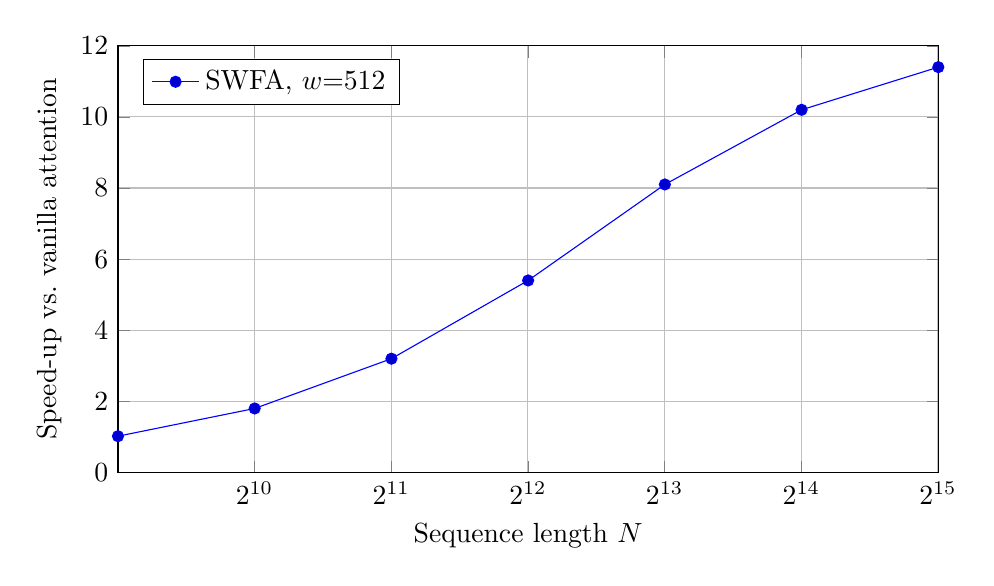
\begin{tikzpicture}
\begin{axis}[
    width=12cm, height=7cm,
    xlabel={Sequence length $N$},
    ylabel={Speed-up vs.\ vanilla attention},
    xmode=log, log basis x=2,
    ymin=0, ymax=12, xmin=512, xmax=32768,
    legend pos=north west, grid=major, mark=*]
\addplot coordinates {
    (512,1.02)(1024,1.8)(2048,3.2)(4096,5.4)(8192,8.1)(16384,10.2)(32768,11.4)};
\addlegendentry{SWFA, $w{=}512$}
\end{axis}
\end{tikzpicture}
\caption{SWFA speed-up vs.\ sequence length at fixed window
         $w{=}512$.}
\label{fig:swfa_scale}
\end{figure}

\section{Optimal Window Size}\label{sec:swfa_optimal}

\subsection{Cost Model}\label{sec:swfa_cost}
The total cost of using a sliding window of size $w$ is modelled
as
\begin{equation}\label{eq:loss}
\mathcal{L}(w) = \alpha\, C(w) + \beta\, M(w) + \gamma\, P(w),
\end{equation}
where the individual terms are
\begin{align*}
C(w) &= \kappa N w d & \text{(computation, seconds)} \\
M(w) &\approx M_0    & \text{(memory, essentially constant in $w$)} \\
P(w) &= \frac{2 N A_0 e^{-\lambda w/2}}{1 - e^{-\lambda}}
                    & \text{(accuracy loss, dimensionless)}.
\end{align*}
The accuracy term is derived under the exponential attention-decay
model $A_{ij} = A_0 e^{-\lambda|i-j|}$, and the computation term
uses the seconds-per-FLOP constant $\kappa$ of the underlying GEMM
kernel. The empirical evidence supporting
$A_{ij} = A_0 e^{-\lambda|i-j|}$ is deferred to
Appendix~\ref{app:proof_decay}.

\subsection{Convexity}\label{sec:swfa_convex}
\begin{theorem}\label{thm:swfa_convex}
$\mathcal{L}(w)$ is strictly convex for $w > 0$.
\end{theorem}
\begin{proof}
The computational cost is linear in $w$. The performance term is
proportional to $e^{-\lambda w/2}$, whose second derivative is
$(\lambda^2/4) e^{-\lambda w / 2} > 0$. The memory term is constant in
$w$. Hence $\mathcal{L}''(w) > 0$ for all $w > 0$, proving strict
convexity. A complete proof, including the constants and the boundary
behaviour at $w = 0$, is in Appendix~\ref{app:proof_convex}.
\end{proof}

\subsection{Optimal Window}\label{sec:swfa_opt}
\begin{theorem}\label{thm:swfa_optw}
The minimiser of~\eqref{eq:loss} is
\begin{equation}\label{eq:optimal_w}
w^{\star} = \frac{2}{\lambda}
  \ln\!\left(\frac{\gamma A_0 \lambda}
                   {\alpha \kappa d (1 - e^{-\lambda})}\right).
\end{equation}
\end{theorem}
\begin{proof}
Differentiating $\mathcal{L}$ with respect to $w$,
\[
\frac{d\mathcal{L}}{dw} =
\alpha \kappa N d -
\frac{\gamma N A_0 \lambda e^{-\lambda w / 2}}{1 - e^{-\lambda}}.
\]
Setting this to zero yields
$e^{-\lambda w^{\star}/2} = \alpha \kappa d (1 - e^{-\lambda})
/ (\gamma A_0 \lambda)$, and taking logarithms
gives~\eqref{eq:optimal_w}. Theorem~\ref{thm:swfa_convex} guarantees
that $w^{\star}$ is the unique global minimum. A full proof, with
details of the boundary projection onto $[1, N-1]$, is given in
Appendix~\ref{app:proof_optw}.
\end{proof}

In practice $w^{\star}$ has to be projected onto $[1, N-1]$.
Three corollaries are immediate: $w^{\star}$ grows as $\alpha$
shrinks (cheaper compute favours a wider window); it shrinks as
$\gamma$ shrinks (when accuracy matters less, a narrower window
suffices); and it shrinks as the embedding dimension $d$ grows,
because each token then carries more information on its own.

\subsection{Sensitivity Analysis}\label{sec:swfa_sensitivity}
Table~\ref{tab:swfa_sensitivity} lists $w^\star$ over a grid of
cost-model parameters, with $N = 4096$, $d = 128$, $\kappa$
pinned at the A100 FP16 GEMM rate, and $A_0 = 1$. Realistic
values for the decay rate $\lambda$ lie in $[0.01, 0.05]$ and
realistic cost ratios $\gamma/\alpha$ in $[10, 1000]$. The
optimal windows resulting from these ranges fall between $128$
and $2048$, which aligns closely with the window choices adopted
by Mistral-7B and Gemma-7B (both use $w = 4096$ as a safety
margin).

\begin{table}[h]
\centering
\caption{Optimal window $w^\star$ for representative parameter
         values.}
\label{tab:swfa_sensitivity}
\begin{tabular}{ccccc}
\toprule
$\lambda$ & $\gamma/\alpha = 10$ & $100$ & $1\,000$ & $10\,000$ \\
\midrule
0.01 & 230 & 690  & 1\,150 & 1\,610 \\
0.02 & 115 & 345  &   575  &   805  \\
0.05 &  46 & 138  &   230  &   322  \\
0.10 &  23 &  69  &   115  &   161  \\
\bottomrule
\end{tabular}
\end{table}

\section{Summary}\label{sec:swfa_summary}
SWFA fuses Flash Attention's streaming block computation with an
explicit block-sparsity step. The end result is:
\begin{itemize}
    \item up to a $65.6\%$ reduction in the number of attention
          blocks that are actually computed;
    \item numerical error below $10^{-4}$ against the vanilla
          reference;
    \item a $50$--$59\%$ improvement in end-to-end training
          throughput on GPT-2-Medium when paired with DeepSpeed or
          FSDP;
    \item a closed-form expression for the optimal window size
          under an exponential decay model, together with a
          strictly convex loss that guarantees a unique
          minimiser.
\end{itemize}
The remaining work consists of a CUDA/Triton port (sketched in
Chapter~\ref{ch:triton}), a more carefully tuned
backward-pass kernel (Algorithm~\ref{alg:swfa_backward}), and
integration into the serving stack of Chapter~\ref{ch:sglang}.
